% Final presentation (15 min + 5 min Q&A). Numbers come only from the manuscript's generated macros.
\documentclass[aspectratio=169,10pt]{beamer}
\usetheme{default}
\usecolortheme{dove}
\setbeamertemplate{navigation symbols}{}
\setbeamertemplate{footline}[frame number]
\setbeamerfont{frametitle}{series=\bfseries}
\usepackage{booktabs,graphicx,tikz}
\usetikzlibrary{positioning,arrows.meta}
\graphicspath{{../manuscript/corrected/generated/}}
% AUTO-GENERATED by phishresearch.reporting - do not edit
\makeatletter
\newcommand{\res}[1]{\@ifundefined{r@#1}{\textbf{??#1??}}{\@nameuse{r@#1}}}
\@namedef{r@freezeHash}{069912e332d7}
\@namedef{r@nBoot}{2,000}
\@namedef{r@nAn}{73,575}
\@namedef{r@cAn}{46,769}
\@namedef{r@nAbenign}{36,400}
\@namedef{r@cAbenign}{22,167}
\@namedef{r@nAphishing}{37,175}
\@namedef{r@cAphishing}{24,602}
\@namedef{r@dupA}{18,811}
\@namedef{r@quarA}{3}
\@namedef{r@purgeA}{7,992}
\@namedef{r@lossBenignA}{25.9}
\@namedef{r@lossPhishA}{1.0}
\@namedef{r@groupsA}{20,913}
\@namedef{r@topGroupA}{wikipedia.org}
\@namedef{r@topGroupShareA}{2.9}
\@namedef{r@nBn}{92,500}
\@namedef{r@cBn}{75,077}
\@namedef{r@nBbenign}{46,250}
\@namedef{r@cBbenign}{29,758}
\@namedef{r@nBphishing}{46,250}
\@namedef{r@cBphishing}{45,319}
\@namedef{r@dupB}{1}
\@namedef{r@quarB}{17}
\@namedef{r@purgeB}{17,405}
\@namedef{r@lossBenignB}{35.6}
\@namedef{r@lossPhishB}{2.0}
\@namedef{r@groupsB}{6,735}
\@namedef{r@topGroupB}{za.com}
\@namedef{r@topGroupShareB}{11.0}
\@namedef{r@sharedGroups}{692}
\@namedef{r@exactOverlap}{33}
\@namedef{r@labelJoin}{73,575}
\@namedef{r@labelAgree}{100.0}
\@namedef{r@splitAFIT}{28,061}
\@namedef{r@splitGroupsAFIT}{8,018}
\@namedef{r@splitAVAL}{9,355}
\@namedef{r@splitGroupsAVAL}{6,448}
\@namedef{r@splitATEST}{9,353}
\@namedef{r@splitGroupsATEST}{6,447}
\@namedef{r@splitBFIT}{45,050}
\@namedef{r@splitGroupsBFIT}{2,614}
\@namedef{r@splitBVAL}{15,014}
\@namedef{r@splitGroupsBVAL}{2,060}
\@namedef{r@splitBTEST}{15,013}
\@namedef{r@splitGroupsBTEST}{2,061}
\@namedef{r@F1AARFALL}{0.895}
\@namedef{r@F1loAARFALL}{0.887}
\@namedef{r@F1hiAARFALL}{0.902}
\@namedef{r@APAARFALL}{0.962}
\@namedef{r@RecAARFALL}{0.475}
\@namedef{r@FPRAARFALL}{0.7}
\@namedef{r@F1dbAARFALL}{0.862}
\@namedef{r@F1AARFMEANPIbudget}{0.897}
\@namedef{r@F1loAARFMEANPIbudget}{0.889}
\@namedef{r@F1hiAARFMEANPIbudget}{0.904}
\@namedef{r@APAARFMEANPIbudget}{0.962}
\@namedef{r@RecAARFMEANPIbudget}{0.478}
\@namedef{r@FPRAARFMEANPIbudget}{0.8}
\@namedef{r@F1dbAARFMEANPIbudget}{0.865}
\@namedef{r@F1AARFSTABLEPIbudget}{0.896}
\@namedef{r@F1loAARFSTABLEPIbudget}{0.889}
\@namedef{r@F1hiAARFSTABLEPIbudget}{0.903}
\@namedef{r@APAARFSTABLEPIbudget}{0.962}
\@namedef{r@RecAARFSTABLEPIbudget}{0.468}
\@namedef{r@FPRAARFSTABLEPIbudget}{0.7}
\@namedef{r@F1dbAARFSTABLEPIbudget}{0.864}
\@namedef{r@F1AALGBMALL}{0.902}
\@namedef{r@F1loAALGBMALL}{0.894}
\@namedef{r@F1hiAALGBMALL}{0.909}
\@namedef{r@APAALGBMALL}{0.966}
\@namedef{r@RecAALGBMALL}{0.559}
\@namedef{r@FPRAALGBMALL}{0.9}
\@namedef{r@F1dbAALGBMALL}{0.872}
\@namedef{r@F1AALGBMMEANPIbudget}{0.900}
\@namedef{r@F1loAALGBMMEANPIbudget}{0.893}
\@namedef{r@F1hiAALGBMMEANPIbudget}{0.908}
\@namedef{r@APAALGBMMEANPIbudget}{0.965}
\@namedef{r@RecAALGBMMEANPIbudget}{0.553}
\@namedef{r@FPRAALGBMMEANPIbudget}{1.0}
\@namedef{r@F1dbAALGBMMEANPIbudget}{0.873}
\@namedef{r@F1AALGBMSTABLEPIbudget}{0.900}
\@namedef{r@F1loAALGBMSTABLEPIbudget}{0.892}
\@namedef{r@F1hiAALGBMSTABLEPIbudget}{0.907}
\@namedef{r@APAALGBMSTABLEPIbudget}{0.965}
\@namedef{r@RecAALGBMSTABLEPIbudget}{0.549}
\@namedef{r@FPRAALGBMSTABLEPIbudget}{1.0}
\@namedef{r@F1dbAALGBMSTABLEPIbudget}{0.873}
\@namedef{r@F1ABRFALL}{0.917}
\@namedef{r@F1loABRFALL}{0.905}
\@namedef{r@F1hiABRFALL}{0.929}
\@namedef{r@APABRFALL}{0.947}
\@namedef{r@RecABRFALL}{0.017}
\@namedef{r@FPRABRFALL}{0.3}
\@namedef{r@F1dbABRFALL}{0.782}
\@namedef{r@F1ABRFMEANPIbudget}{0.914}
\@namedef{r@F1loABRFMEANPIbudget}{0.901}
\@namedef{r@F1hiABRFMEANPIbudget}{0.925}
\@namedef{r@APABRFMEANPIbudget}{0.947}
\@namedef{r@RecABRFMEANPIbudget}{0.017}
\@namedef{r@FPRABRFMEANPIbudget}{0.3}
\@namedef{r@F1dbABRFMEANPIbudget}{0.767}
\@namedef{r@F1ABRFSTABLEPIbudget}{0.913}
\@namedef{r@F1loABRFSTABLEPIbudget}{0.901}
\@namedef{r@F1hiABRFSTABLEPIbudget}{0.924}
\@namedef{r@APABRFSTABLEPIbudget}{0.950}
\@namedef{r@RecABRFSTABLEPIbudget}{0.016}
\@namedef{r@FPRABRFSTABLEPIbudget}{0.2}
\@namedef{r@F1dbABRFSTABLEPIbudget}{0.763}
\@namedef{r@F1ABLGBMALL}{0.922}
\@namedef{r@F1loABLGBMALL}{0.910}
\@namedef{r@F1hiABLGBMALL}{0.933}
\@namedef{r@APABLGBMALL}{0.958}
\@namedef{r@RecABLGBMALL}{0.345}
\@namedef{r@FPRABLGBMALL}{1.6}
\@namedef{r@F1dbABLGBMALL}{0.796}
\@namedef{r@F1ABLGBMMEANPIbudget}{0.916}
\@namedef{r@F1loABLGBMMEANPIbudget}{0.903}
\@namedef{r@F1hiABLGBMMEANPIbudget}{0.927}
\@namedef{r@APABLGBMMEANPIbudget}{0.956}
\@namedef{r@RecABLGBMMEANPIbudget}{0.510}
\@namedef{r@FPRABLGBMMEANPIbudget}{1.8}
\@namedef{r@F1dbABLGBMMEANPIbudget}{0.778}
\@namedef{r@F1ABLGBMSTABLEPIbudget}{0.915}
\@namedef{r@F1loABLGBMSTABLEPIbudget}{0.902}
\@namedef{r@F1hiABLGBMSTABLEPIbudget}{0.927}
\@namedef{r@APABLGBMSTABLEPIbudget}{0.956}
\@namedef{r@RecABLGBMSTABLEPIbudget}{0.482}
\@namedef{r@FPRABLGBMSTABLEPIbudget}{1.7}
\@namedef{r@F1dbABLGBMSTABLEPIbudget}{0.776}
\@namedef{r@F1BBRFALL}{0.956}
\@namedef{r@F1loBBRFALL}{0.947}
\@namedef{r@F1hiBBRFALL}{0.964}
\@namedef{r@APBBRFALL}{0.993}
\@namedef{r@RecBBRFALL}{0.831}
\@namedef{r@FPRBBRFALL}{0.4}
\@namedef{r@F1dbBBRFALL}{0.916}
\@namedef{r@F1BBRFMEANPIbudget}{0.941}
\@namedef{r@F1loBBRFMEANPIbudget}{0.930}
\@namedef{r@F1hiBBRFMEANPIbudget}{0.950}
\@namedef{r@APBBRFMEANPIbudget}{0.989}
\@namedef{r@RecBBRFMEANPIbudget}{0.823}
\@namedef{r@FPRBBRFMEANPIbudget}{0.6}
\@namedef{r@F1dbBBRFMEANPIbudget}{0.888}
\@namedef{r@F1BBRFSTABLEPIbudget}{0.944}
\@namedef{r@F1loBBRFSTABLEPIbudget}{0.933}
\@namedef{r@F1hiBBRFSTABLEPIbudget}{0.953}
\@namedef{r@APBBRFSTABLEPIbudget}{0.989}
\@namedef{r@RecBBRFSTABLEPIbudget}{0.820}
\@namedef{r@FPRBBRFSTABLEPIbudget}{0.8}
\@namedef{r@F1dbBBRFSTABLEPIbudget}{0.904}
\@namedef{r@F1BBLGBMALL}{0.958}
\@namedef{r@F1loBBLGBMALL}{0.949}
\@namedef{r@F1hiBBLGBMALL}{0.966}
\@namedef{r@APBBLGBMALL}{0.993}
\@namedef{r@RecBBLGBMALL}{0.876}
\@namedef{r@FPRBBLGBMALL}{0.5}
\@namedef{r@F1dbBBLGBMALL}{0.936}
\@namedef{r@F1BBLGBMMEANPIbudget}{0.942}
\@namedef{r@F1loBBLGBMMEANPIbudget}{0.932}
\@namedef{r@F1hiBBLGBMMEANPIbudget}{0.951}
\@namedef{r@APBBLGBMMEANPIbudget}{0.990}
\@namedef{r@RecBBLGBMMEANPIbudget}{0.820}
\@namedef{r@FPRBBLGBMMEANPIbudget}{0.2}
\@namedef{r@F1dbBBLGBMMEANPIbudget}{0.871}
\@namedef{r@F1BBLGBMSTABLEPIbudget}{0.946}
\@namedef{r@F1loBBLGBMSTABLEPIbudget}{0.937}
\@namedef{r@F1hiBBLGBMSTABLEPIbudget}{0.955}
\@namedef{r@APBBLGBMSTABLEPIbudget}{0.990}
\@namedef{r@RecBBLGBMSTABLEPIbudget}{0.821}
\@namedef{r@FPRBBLGBMSTABLEPIbudget}{0.3}
\@namedef{r@F1dbBBLGBMSTABLEPIbudget}{0.895}
\@namedef{r@F1BARFALL}{0.739}
\@namedef{r@F1loBARFALL}{0.727}
\@namedef{r@F1hiBARFALL}{0.751}
\@namedef{r@APBARFALL}{0.829}
\@namedef{r@RecBARFALL}{0.115}
\@namedef{r@FPRBARFALL}{1.4}
\@namedef{r@F1dbBARFALL}{0.703}
\@namedef{r@F1BARFMEANPIbudget}{0.639}
\@namedef{r@F1loBARFMEANPIbudget}{0.625}
\@namedef{r@F1hiBARFMEANPIbudget}{0.652}
\@namedef{r@APBARFMEANPIbudget}{0.739}
\@namedef{r@RecBARFMEANPIbudget}{0.101}
\@namedef{r@FPRBARFMEANPIbudget}{2.2}
\@namedef{r@F1dbBARFMEANPIbudget}{0.604}
\@namedef{r@F1BARFSTABLEPIbudget}{0.697}
\@namedef{r@F1loBARFSTABLEPIbudget}{0.685}
\@namedef{r@F1hiBARFSTABLEPIbudget}{0.710}
\@namedef{r@APBARFSTABLEPIbudget}{0.746}
\@namedef{r@RecBARFSTABLEPIbudget}{0.135}
\@namedef{r@FPRBARFSTABLEPIbudget}{3.1}
\@namedef{r@F1dbBARFSTABLEPIbudget}{0.649}
\@namedef{r@F1BALGBMALL}{0.790}
\@namedef{r@F1loBALGBMALL}{0.779}
\@namedef{r@F1hiBALGBMALL}{0.800}
\@namedef{r@APBALGBMALL}{0.883}
\@namedef{r@RecBALGBMALL}{0.440}
\@namedef{r@FPRBALGBMALL}{3.2}
\@namedef{r@F1dbBALGBMALL}{0.747}
\@namedef{r@F1BALGBMMEANPIbudget}{0.619}
\@namedef{r@F1loBALGBMMEANPIbudget}{0.605}
\@namedef{r@F1hiBALGBMMEANPIbudget}{0.634}
\@namedef{r@APBALGBMMEANPIbudget}{0.772}
\@namedef{r@RecBALGBMMEANPIbudget}{0.143}
\@namedef{r@FPRBALGBMMEANPIbudget}{0.9}
\@namedef{r@F1dbBALGBMMEANPIbudget}{0.588}
\@namedef{r@F1BALGBMSTABLEPIbudget}{0.697}
\@namedef{r@F1loBALGBMSTABLEPIbudget}{0.685}
\@namedef{r@F1hiBALGBMSTABLEPIbudget}{0.709}
\@namedef{r@APBALGBMSTABLEPIbudget}{0.790}
\@namedef{r@RecBALGBMSTABLEPIbudget}{0.220}
\@namedef{r@FPRBALGBMSTABLEPIbudget}{2.2}
\@namedef{r@F1dbBALGBMSTABLEPIbudget}{0.653}
\@namedef{r@DropALGBMALL}{-2.0}
\@namedef{r@DropALGBMMEANPIbudget}{-1.5}
\@namedef{r@DropALGBMMEANPImatched}{-1.5}
\@namedef{r@DropALGBMSTABLEPIbudget}{-1.6}
\@namedef{r@DropALGBMSTABLEPImatched}{-1.6}
\@namedef{r@DropARFALL}{-2.3}
\@namedef{r@DropARFMEANPIbudget}{-1.7}
\@namedef{r@DropARFMEANPImatched}{-1.7}
\@namedef{r@DropARFSTABLEPIbudget}{-1.7}
\@namedef{r@DropARFSTABLEPImatched}{-1.7}
\@namedef{r@DropBLGBMALL}{16.9}
\@namedef{r@DropBLGBMMEANPIbudget}{32.3}
\@namedef{r@DropBLGBMMEANPImatched}{32.3}
\@namedef{r@DropBLGBMSTABLEPIbudget}{25.0}
\@namedef{r@DropBLGBMSTABLEPImatched}{25.0}
\@namedef{r@DropBRFALL}{21.7}
\@namedef{r@DropBRFMEANPIbudget}{30.2}
\@namedef{r@DropBRFMEANPImatched}{30.2}
\@namedef{r@DropBRFSTABLEPIbudget}{24.7}
\@namedef{r@DropBRFSTABLEPImatched}{24.7}
\@namedef{r@DropMin}{-2.3}
\@namedef{r@DropMax}{21.7}
\@namedef{r@DeltaABRF}{-0.000}
\@namedef{r@DeltaLoABRF}{-0.001}
\@namedef{r@DeltaHiABRF}{+0.000}
\@namedef{r@DeltaABLGBM}{-0.000}
\@namedef{r@DeltaLoABLGBM}{-0.001}
\@namedef{r@DeltaHiABLGBM}{+0.000}
\@namedef{r@DeltaBARF}{+0.059}
\@namedef{r@DeltaLoBARF}{+0.051}
\@namedef{r@DeltaHiBARF}{+0.066}
\@namedef{r@DeltaBALGBM}{+0.077}
\@namedef{r@DeltaLoBALGBM}{+0.069}
\@namedef{r@DeltaHiBALGBM}{+0.086}
\@namedef{r@nPrimaryExcl}{2}
\@namedef{r@nPrimaryPos}{2}
\@namedef{r@nPrimaryEff}{2}
\@namedef{r@SecABRFSTABLEALL}{-0.004}
\@namedef{r@SecABRFMEANALL}{-0.004}
\@namedef{r@SecABRFSTABLE}{-0.000}
\@namedef{r@SecABLGBMSTABLEALL}{-0.007}
\@namedef{r@SecABLGBMMEANALL}{-0.006}
\@namedef{r@SecABLGBMSTABLE}{-0.000}
\@namedef{r@SecBARFSTABLEALL}{-0.042}
\@namedef{r@SecBARFMEANALL}{-0.100}
\@namedef{r@SecBARFSTABLE}{+0.059}
\@namedef{r@SecBALGBMSTABLEALL}{-0.093}
\@namedef{r@SecBALGBMMEANALL}{-0.170}
\@namedef{r@SecBALGBMSTABLE}{+0.077}
\@namedef{r@highCorrA}{14}
\@namedef{r@piSecA}{26.1}
\@namedef{r@highCorrB}{17}
\@namedef{r@piSecB}{10.6}
\@namedef{r@relLatB1Min}{0.75}
\@namedef{r@relLatB1Max}{1.10}
\@namedef{r@relLatBkMin}{0.47}
\@namedef{r@relLatBkMax}{1.01}
\@namedef{r@extractShareMedian}{10.4}
\@namedef{r@cpu}{Intel64 Family 6 Model 154 Stepping 3, GenuineIntel}
\@namedef{r@ram}{32}
\@namedef{r@pyver}{3.10.0}
\@namedef{r@RhoALGBMALL}{0.99}
\@namedef{r@RhoALGBMSTABLEPIbudget}{0.88}
\@namedef{r@RhoARFALL}{0.97}
\@namedef{r@RhoARFSTABLEPIbudget}{0.81}
\@namedef{r@RhoBLGBMALL}{0.96}
\@namedef{r@RhoBLGBMSTABLEPIbudget}{0.98}
\@namedef{r@RhoBRFALL}{0.95}
\@namedef{r@RhoBRFSTABLEPIbudget}{0.98}
\@namedef{r@shapAddErr}{2.9e-08}
\@namedef{r@rhoMin}{0.81}
\@namedef{r@rhoMax}{0.99}
\@namedef{r@rhoSeedMin}{1.00}
\@namedef{r@medLenABenign}{55}
\@namedef{r@medDotsABenign}{2}
\@namedef{r@medSubABenign}{1}
\@namedef{r@httpsABenign}{34.9}
\@namedef{r@medLenAPhish}{63}
\@namedef{r@medDotsAPhish}{2}
\@namedef{r@medSubAPhish}{0}
\@namedef{r@httpsAPhish}{1.5}
\@namedef{r@medLenBBenign}{41}
\@namedef{r@medDotsBBenign}{2}
\@namedef{r@medSubBBenign}{1}
\@namedef{r@httpsBBenign}{83.5}
\@namedef{r@medLenBPhish}{74}
\@namedef{r@medDotsBPhish}{5}
\@namedef{r@medSubBPhish}{3}
\@namedef{r@httpsBPhish}{30.6}
\@namedef{r@status}{benchmark: completed, evaluation: completed, shap: completed}
\makeatother

% AUTO-GENERATED by phishresearch.extensions.report from extensions/run_20261116T063740629948Z_fe541b37 - do not edit
\makeatletter
\@namedef{r@xRuleSrcA}{0.739}
\@namedef{r@xRuleTgtA}{0.874}
\@namedef{r@xRuleTgtAPA}{0.858}
\@namedef{r@xRuleTgtAUCA}{0.855}
\@namedef{r@xRuleTgtRecA}{0.845}
\@namedef{r@xRuleTgtFPRA}{13.5}
\@namedef{r@xLRSrcA}{0.871}
\@namedef{r@xLRTgtA}{0.275}
\@namedef{r@xLRTgtAPA}{0.840}
\@namedef{r@xLRTgtAUCA}{0.847}
\@namedef{r@xLRTgtRecA}{0.168}
\@namedef{r@xLRTgtFPRA}{8.6}
\@namedef{r@xRFSrcA}{0.903}
\@namedef{r@xRFTgtA}{0.918}
\@namedef{r@xRFTgtAPA}{0.966}
\@namedef{r@xRFTgtAUCA}{0.961}
\@namedef{r@xRFTgtRecA}{0.891}
\@namedef{r@xRFTgtFPRA}{7.7}
\@namedef{r@xLGBMSrcA}{0.909}
\@namedef{r@xLGBMTgtA}{0.928}
\@namedef{r@xLGBMTgtAPA}{0.972}
\@namedef{r@xLGBMTgtAUCA}{0.968}
\@namedef{r@xLGBMTgtRecA}{0.898}
\@namedef{r@xLGBMTgtFPRA}{5.7}
\@namedef{r@xRFnoHSrcA}{0.897}
\@namedef{r@xRFnoHTgtA}{0.898}
\@namedef{r@xRFnoHTgtAPA}{0.921}
\@namedef{r@xRFnoHTgtAUCA}{0.933}
\@namedef{r@xRFnoHTgtRecA}{0.958}
\@namedef{r@xRFnoHTgtFPRA}{26.7}
\@namedef{r@xLGBMnoHSrcA}{0.899}
\@namedef{r@xLGBMnoHTgtA}{0.906}
\@namedef{r@xLGBMnoHTgtAPA}{0.946}
\@namedef{r@xLGBMnoHTgtAUCA}{0.942}
\@namedef{r@xLGBMnoHTgtRecA}{0.947}
\@namedef{r@xLGBMnoHTgtFPRA}{21.9}
\@namedef{r@xRuleSrcB}{0.874}
\@namedef{r@xRuleTgtB}{0.739}
\@namedef{r@xRuleTgtAPB}{0.593}
\@namedef{r@xRuleTgtAUCB}{0.618}
\@namedef{r@xRuleTgtRecB}{0.976}
\@namedef{r@xRuleTgtFPRB}{74.0}
\@namedef{r@xLRSrcB}{0.929}
\@namedef{r@xLRTgtB}{0.666}
\@namedef{r@xLRTgtAPB}{0.749}
\@namedef{r@xLRTgtAUCB}{0.763}
\@namedef{r@xLRTgtRecB}{0.589}
\@namedef{r@xLRTgtFPRB}{19.9}
\@namedef{r@xRFSrcB}{0.951}
\@namedef{r@xRFTgtB}{0.734}
\@namedef{r@xRFTgtAPB}{0.826}
\@namedef{r@xRFTgtAUCB}{0.821}
\@namedef{r@xRFTgtRecB}{0.672}
\@namedef{r@xRFTgtFPRB}{17.6}
\@namedef{r@xLGBMSrcB}{0.955}
\@namedef{r@xLGBMTgtB}{0.783}
\@namedef{r@xLGBMTgtAPB}{0.874}
\@namedef{r@xLGBMTgtAUCB}{0.863}
\@namedef{r@xLGBMTgtRecB}{0.772}
\@namedef{r@xLGBMTgtFPRB}{22.1}
\@namedef{r@xRFnoHSrcB}{0.951}
\@namedef{r@xRFnoHTgtB}{0.692}
\@namedef{r@xRFnoHTgtAPB}{0.812}
\@namedef{r@xRFnoHTgtAUCB}{0.792}
\@namedef{r@xRFnoHTgtRecB}{0.598}
\@namedef{r@xRFnoHTgtFPRB}{14.6}
\@namedef{r@xLGBMnoHSrcB}{0.956}
\@namedef{r@xLGBMnoHTgtB}{0.716}
\@namedef{r@xLGBMnoHTgtAPB}{0.852}
\@namedef{r@xLGBMnoHTgtAUCB}{0.834}
\@namedef{r@xLGBMnoHTgtRecB}{0.638}
\@namedef{r@xLGBMnoHTgtFPRB}{16.0}
\@namedef{r@xDsRFLRA}{+0.032}
\@namedef{r@xDsRFLRACI}{[+0.026, +0.038]}
\@namedef{r@xDRFLRA}{+0.643}
\@namedef{r@xDRFLRACI}{[+0.611, +0.674]}
\@namedef{r@xDsLGBMLRA}{+0.037}
\@namedef{r@xDsLGBMLRACI}{[+0.031, +0.044]}
\@namedef{r@xDLGBMLRA}{+0.653}
\@namedef{r@xDLGBMLRACI}{[+0.622, +0.682]}
\@namedef{r@xDsRFnoHA}{+0.007}
\@namedef{r@xDsRFnoHACI}{[+0.003, +0.010]}
\@namedef{r@xDRFnoHA}{+0.020}
\@namedef{r@xDRFnoHACI}{[+0.007, +0.032]}
\@namedef{r@xDsLGBMnoHA}{+0.010}
\@namedef{r@xDsLGBMnoHACI}{[+0.006, +0.014]}
\@namedef{r@xDLGBMnoHA}{+0.022}
\@namedef{r@xDLGBMnoHACI}{[+0.010, +0.034]}
\@namedef{r@xDsRFLRB}{+0.022}
\@namedef{r@xDsRFLRBCI}{[+0.014, +0.030]}
\@namedef{r@xDRFLRB}{+0.068}
\@namedef{r@xDRFLRBCI}{[+0.055, +0.080]}
\@namedef{r@xDsLGBMLRB}{+0.027}
\@namedef{r@xDsLGBMLRBCI}{[+0.018, +0.034]}
\@namedef{r@xDLGBMLRB}{+0.117}
\@namedef{r@xDLGBMLRBCI}{[+0.104, +0.131]}
\@namedef{r@xDsRFnoHB}{-0.000}
\@namedef{r@xDsRFnoHBCI}{[-0.002, +0.001]}
\@namedef{r@xDRFnoHB}{+0.042}
\@namedef{r@xDRFnoHBCI}{[+0.037, +0.048]}
\@namedef{r@xDsLGBMnoHB}{-0.001}
\@namedef{r@xDsLGBMnoHBCI}{[-0.003, +0.001]}
\@namedef{r@xDLGBMnoHB}{+0.067}
\@namedef{r@xDLGBMnoHBCI}{[+0.060, +0.075]}
\@namedef{r@xAHttpsHTTPSFPR}{1.9}
\@namedef{r@xAHttpsHTTPSFNR}{57.4}
\@namedef{r@xAHttpsHTTPSShare}{44}
\@namedef{r@xAHttpsnotHTTPSFPR}{30.2}
\@namedef{r@xAHttpsnotHTTPSFNR}{1.6}
\@namedef{r@xAHttpsnotHTTPSShare}{56}
\@namedef{r@xASub0FPR}{7.5}
\@namedef{r@xASub0FNR}{35.5}
\@namedef{r@xASub0Share}{19}
\@namedef{r@xASub1FPR}{4.0}
\@namedef{r@xASub1FNR}{49.4}
\@namedef{r@xASub1Share}{33}
\@namedef{r@xASubge2FPR}{22.6}
\@namedef{r@xASubge2FNR}{0.6}
\@namedef{r@xASubge2Share}{48}
\@namedef{r@xBHttpsHTTPSFPR}{11.7}
\@namedef{r@xBHttpsHTTPSFNR}{33.3}
\@namedef{r@xBHttpsHTTPSShare}{14}
\@namedef{r@xBHttpsnotHTTPSFPR}{25.7}
\@namedef{r@xBHttpsnotHTTPSFNR}{22.5}
\@namedef{r@xBHttpsnotHTTPSShare}{86}
\@namedef{r@xBSub0FPR}{51.9}
\@namedef{r@xBSub0FNR}{10.5}
\@namedef{r@xBSub0Share}{49}
\@namedef{r@xBSub1FPR}{10.9}
\@namedef{r@xBSub1FNR}{53.2}
\@namedef{r@xBSub1Share}{49}
\@namedef{r@xBSubge2FPR}{18.8}
\@namedef{r@xBSubge2FNR}{13.4}
\@namedef{r@xBSubge2Share}{2}
\@namedef{r@xdF01A}{+0.44}
\@namedef{r@xdF01B}{+0.72}
\@namedef{r@xdF02A}{+0.12}
\@namedef{r@xdF02B}{+2.11}
\@namedef{r@xdF03A}{+0.04}
\@namedef{r@xdF03B}{+0.09}
\@namedef{r@xdF06A}{+0.39}
\@namedef{r@xdF06B}{+1.75}
\@namedef{r@xdF07A}{-0.61}
\@namedef{r@xdF07B}{-0.17}
\@namedef{r@xdF16A}{+0.55}
\@namedef{r@xdF16B}{+0.16}
\@namedef{r@xdF18A}{+0.54}
\@namedef{r@xdF18B}{+0.03}
\@namedef{r@xdF20A}{+0.42}
\@namedef{r@xdF20B}{+1.04}
\@namedef{r@xdF22A}{-0.38}
\@namedef{r@xdF22B}{+1.43}
\@namedef{r@xdF23A}{-0.58}
\@namedef{r@xdF23B}{+1.54}
\@namedef{r@xdF29A}{+0.74}
\@namedef{r@xdF29B}{-0.34}
\@namedef{r@xdF30A}{-0.98}
\@namedef{r@xdF30B}{-1.23}
\@namedef{r@xdF35A}{+0.77}
\@namedef{r@xdF35B}{+0.29}
\@namedef{r@xdF36A}{+0.51}
\@namedef{r@xdF36B}{+0.18}
\@namedef{r@xFlipList}{\texttt{host\_label\_count}, \texttt{subdomain\_label\_count}, \texttt{has\_query}}
\@namedef{r@xNFlip}{3}
\@namedef{r@xNEda}{14}
\@namedef{r@xHttpsBenignA}{34.9}
\@namedef{r@xHttpsPhishA}{1.5}
\@namedef{r@xHttpsBenignB}{83.5}
\@namedef{r@xHttpsPhishB}{30.6}
\makeatother

\definecolor{acc}{HTML}{2a78d6}
\definecolor{warn}{HTML}{eb6834}
\newcommand{\key}[1]{{\color{acc}\textbf{#1}}}

\title{Do Stable Features Transfer?}
\subtitle{Source-Only Feature Selection for Cross-Dataset Phishing URL Detection}
\author{[TEAM MEMBER 1 FULL NAME] \and [TEAM MEMBER 2 FULL NAME]}
\institute{Project category: General Machine Learning (application project)}
\date{}

\begin{document}

\begin{frame}
\titlepage
\end{frame}

% ------------------------------------------------------------------ MOTIVATION
\section{Motivation}
\begin{frame}{Motivation: detectors are trained on one collection, used on another}
\begin{itemize}
\item URL-based phishing filters block a link \emph{before} the page loads: no fetch, no DNS, no third-party lookup.
\item They are trained on whatever labelled dataset exists, then deployed on \key{different traffic}: other brands, hosts, periods, benign populations.
\item Published accuracies are mostly \emph{within} one collection.
\end{itemize}
\vspace{1em}
\begin{block}{Goal}
Measure how much accuracy survives on a dataset the model was \key{never fitted, selected or calibrated on}, and whether choosing \key{stable} features keeps more of it than choosing \key{important} ones, at the same feature budget and lower cost.
\end{block}
\end{frame}

\begin{frame}{Research questions}
\begin{description}[RQ5]
\item[RQ1] How far do RF and LightGBM drop on another source with disjoint domains?
\item[RQ2] Does \key{STABLE-PI} transfer better than \key{MEAN-PI} at the same $k$, and versus all 37 features?
\item[RQ3] Does a smaller feature set measurably reduce detection cost?
\item[RQ4] Which features do the models rely on, source vs.\ target? (SHAP)
\item[RQ5] \emph{(exploratory)} \key{Why} does transfer fail where it does? Baselines, ablation, error analysis.
\end{description}
\vspace{1em}
\small Constraint throughout: \textbf{no target data} for fitting, feature selection or thresholds.
\end{frame}

% ------------------------------------------------------------------ RELATED WORK
\section{Related Work}
\begin{frame}{Related work and gap}
\small
\begin{tabular}{p{0.24\linewidth}p{0.33\linewidth}p{0.33\linewidth}}
\toprule
Study & What it does & What we do differently \\
\midrule
S\'anchez-Paniagua et al.\ 2022 (IEEE Access) & RF, LightGBM, TF-IDF+LR on URL data; legitimate-login representativeness & Other datasets; transfer between collections; no replication claim \\
Rashid et al.\ 2024 (Computer Networks) & Cross-dataset transfer; \key{UDA} uses unlabelled target data; HP dataset & \key{No} target data at all; domain-disjoint splits; both directions \\
Misiek \& Hyla 2026; Kanon et al.\ 2026 & Feature stability across datasets; cost & Stability from \key{one} source only, matched budget \\
\bottomrule
\end{tabular}
\vspace{1em}
\begin{block}{Gap}
Under a strict source-only constraint, does \emph{stability} of importance help transfer at a \emph{matched} budget, and what does compression cost? URL-level random splits leak domains; we split by registered domain.
\end{block}
\end{frame}

% ------------------------------------------------------------------ METHOD
\section{Method}
\begin{frame}{Data: two public collections, made domain-disjoint}
\begin{columns}[T]
\column{0.5\textwidth}
\begin{itemize}
\item \key{EBBU-2017}: \res{nAn} URLs \\ \key{HP} (HISPAR--Phishstats): \res{nBn} URLs
\item Offline canonicalisation; dedup; registered domain via frozen PSL
\item \res{sharedGroups} domains appear in both $\Rightarrow$ \key{removed from both}
\item Cohorts: \res{cAn} (EBBU), \res{cBn} (HP)
\item FIT/VAL/TEST $\approx$ 60/20/20, \key{no domain shared} between partitions
\end{itemize}
\column{0.5\textwidth}
\scriptsize
\resizebox{\linewidth}{!}{\begin{tabular}{llrrr}
\toprule
Source & Stage & URLs & Benign & Phishing \\
\midrule
EBBU-2017 & Loaded & 73,575 & 36,400 & 37,175 \\
EBBU-2017 & Parsed & 73,572 & 36,400 & 37,172 \\
EBBU-2017 & Deduplicated & 54,761 & 29,910 & 24,851 \\
EBBU-2017 & Conflicts removed & 54,761 & 29,910 & 24,851 \\
EBBU-2017 & Cohort (shared domains purged) & 46,769 & 22,167 & 24,602 \\
\midrule
HP & Loaded & 92,500 & 46,250 & 46,250 \\
HP & Parsed & 92,483 & 46,233 & 46,250 \\
HP & Deduplicated & 92,482 & 46,233 & 46,249 \\
HP & Conflicts removed & 92,482 & 46,233 & 46,249 \\
HP & Cohort (shared domains purged) & 75,077 & 29,758 & 45,319 \\
\bottomrule
\end{tabular}
}
\end{columns}
\end{frame}

\begin{frame}{Pipeline (source-only, frozen before TEST)}
\centering
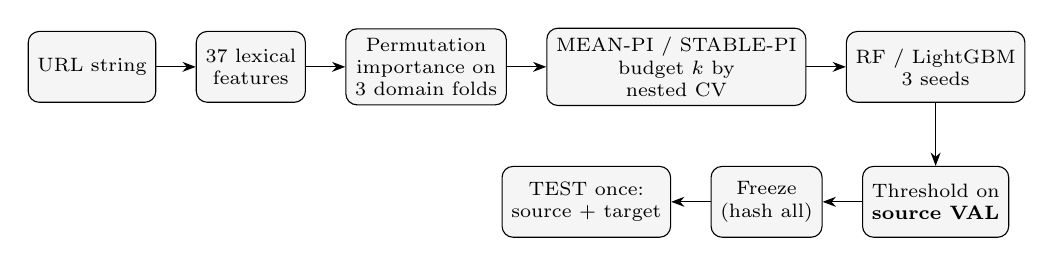
\begin{tikzpicture}[node distance=4mm and 5mm, every node/.style={draw, rounded corners, align=center, font=\scriptsize, minimum height=9mm, fill=gray!8}, >={Stealth}]
\node (u) {URL string};
\node[right=of u] (f) {37 lexical\\features};
\node[right=of f] (pi) {Permutation\\importance on\\3 domain folds};
\node[right=of pi] (sel) {MEAN-PI / STABLE-PI\\budget $k$ by\\nested CV};
\node[right=of sel] (m) {RF / LightGBM\\3 seeds};
\node[below=8mm of m] (t) {Threshold on\\\textbf{source VAL}};
\node[left=of t] (fr) {Freeze\\(hash all)};
\node[left=of fr] (ev) {TEST once:\\source + target};
\draw[->] (u)--(f); \draw[->] (f)--(pi); \draw[->] (pi)--(sel); \draw[->] (sel)--(m); \draw[->] (m)--(t); \draw[->] (t)--(fr); \draw[->] (fr)--(ev);
\end{tikzpicture}
\vspace{6mm}
\begin{itemize}\small
\item \key{MEAN-PI}: rank by mean PI over folds. \key{STABLE-PI}: rank by \#folds in top-12 with PI$>$0, then median PI, rank dispersion.
\item \key{Matched-$k$}: STABLE vs.\ MEAN at the \emph{same} $k$ isolates the ranking rule from the budget.
\item Uncertainty: paired \key{domain-cluster bootstrap} (\res{nBoot} resamples), same resample for both arms.
\end{itemize}
\end{frame}

% ------------------------------------------------------------------ EXPERIMENTS
\section{Experiments}
\begin{frame}{RQ1: transfer is asymmetric}
\centering
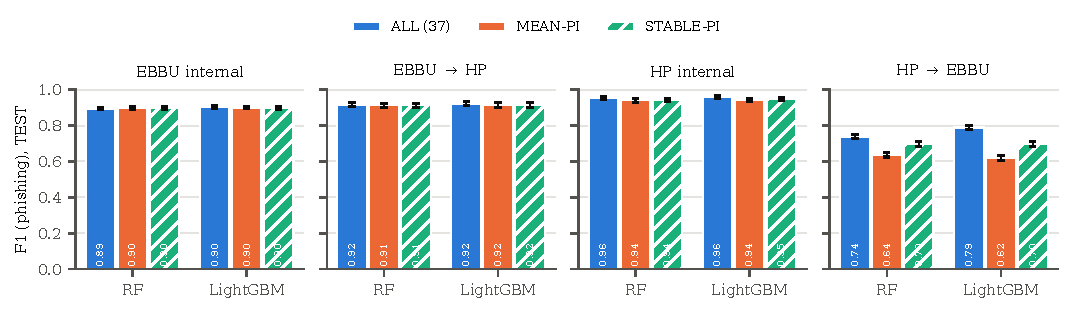
\includegraphics[width=0.95\textwidth]{fig_f1.pdf}
\small
EBBU$\rightarrow$HP: LightGBM F1 \res{F1AALGBMALL} internal $\rightarrow$ \key{\res{F1ABLGBMALL}} on HP (no drop).\quad
HP$\rightarrow$EBBU: \res{F1BBLGBMALL} $\rightarrow$ \textcolor{warn}{\textbf{\res{F1BALGBMALL}}} (drop \res{DropBLGBMALL} pp).
\end{frame}

\begin{frame}{RQ2: does stability help? Only in one direction}
\begin{itemize}
\item Matched-$k$ STABLE-PI $-$ MEAN-PI on target TEST F1 (pre-specified, 4 contrasts):
  \begin{itemize}
  \item HP$\rightarrow$EBBU: RF \key{\res{DeltaBARF}} [\res{DeltaLoBARF}, \res{DeltaHiBARF}], LightGBM \key{\res{DeltaBALGBM}} [\res{DeltaLoBALGBM}, \res{DeltaHiBALGBM}]
  \item EBBU$\rightarrow$HP: RF \res{DeltaABRF}, LightGBM \res{DeltaABLGBM} \;(within the $\pm$0.01 band)
  \end{itemize}
\item But versus \key{ALL 37 features} on HP$\rightarrow$EBBU: STABLE-PI \textcolor{warn}{\res{SecBARFSTABLEALL}} (RF), \textcolor{warn}{\res{SecBALGBMSTABLEALL}} (LightGBM)
\end{itemize}
\begin{alertblock}{Reading}
Stability \emph{reduces the damage} of compression; it does \emph{not} make a compact model transfer as well as ALL.
\end{alertblock}
\end{frame}

\begin{frame}{RQ3: cost savings are modest}
\begin{columns}[T]
\column{0.55\textwidth}
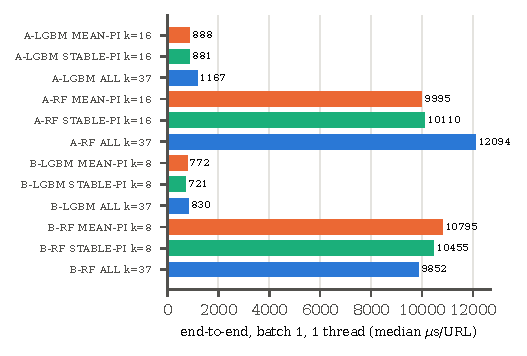
\includegraphics[width=\linewidth]{fig_latency.pdf}
\column{0.45\textwidth}
\small
\begin{itemize}
\item Single URL, 1 thread: reduced subsets take \res{relLatB1Min}--\res{relLatB1Max} of ALL's end-to-end time.
\item Batch 1024, 4 threads: \res{relLatBkMin}--\res{relLatBkMax}.
\item Parsing+extraction = \res{extractShareMedian}\% of single-URL time; tree inference barely depends on $k$.
\end{itemize}
\end{columns}
\end{frame}

\begin{frame}{RQ5: baselines and HTTPS ablation (VAL only, exploratory)}
\centering\scriptsize
\begin{tabular}{lcccccc}
\toprule
& \multicolumn{3}{c}{Source EBBU} & \multicolumn{3}{c}{Source HP} \\
\cmidrule(lr){2-4}\cmidrule(lr){5-7}
Model & F1$_{\mathrm{src}}$ & F1$_{\rightarrow\mathrm{HP}}$ & AP$_{\rightarrow\mathrm{HP}}$ & F1$_{\mathrm{src}}$ & F1$_{\rightarrow\mathrm{EBBU}}$ & AP$_{\rightarrow\mathrm{EBBU}}$ \\
\midrule
Rule: not HTTPS & 0.739 & 0.874 & 0.858 & 0.874 & 0.739 & 0.593 \\
\midrule
LogReg (37) & 0.871 & 0.275 & 0.840 & 0.929 & 0.666 & 0.749 \\
RF (37) v1 & 0.903 & 0.918 & 0.966 & 0.951 & 0.734 & 0.826 \\
LightGBM (37) v1 & 0.909 & 0.928 & 0.972 & 0.955 & 0.783 & 0.874 \\
RF w/o F30 & 0.897 & 0.898 & 0.921 & 0.951 & 0.692 & 0.812 \\
LightGBM w/o F30 & 0.899 & 0.906 & 0.946 & 0.956 & 0.716 & 0.852 \\
\bottomrule
\end{tabular}

\vspace{2mm}
\begin{itemize}\small
\item \key{LogReg}: fine inside a source (\res{xLRSrcA}/\res{xLRSrcB}), but EBBU$\rightarrow$HP F1 \textcolor{warn}{\textbf{\res{xLRTgtA}}} with AUC \res{xLRTgtAUCA}: ranking transfers, \key{threshold does not}.
\item One rule, \key{``not HTTPS $\Rightarrow$ phishing''}, already gets F1 \res{xRuleTgtA} on HP.
\item Removing HTTPS: $\Delta$ source F1 $\approx$ 0, $\Delta$ transfer F1 \res{xDLGBMnoHA} / \res{xDLGBMnoHB} (LightGBM).
\end{itemize}
\end{frame}

\begin{frame}{RQ5: some cues reverse between datasets}
\begin{columns}[T]
\column{0.5\textwidth}
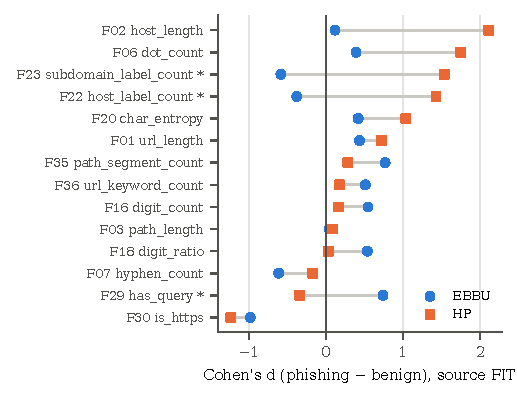
\includegraphics[width=\linewidth]{fig_eda.pdf}
\column{0.5\textwidth}
\small
\begin{itemize}
\item \res{xNFlip}/\res{xNEda} features flip sign: \res{xFlipList}.
\item Subdomain labels: EBBU phishing $d{=}$\res{xdF23A}, HP phishing $d{=}$\res{xdF23B}.
\item HTTPS is shared: \res{xHttpsPhishA}\% / \res{xHttpsPhishB}\% of phishing vs.\ \res{xHttpsBenignA}\% / \res{xHttpsBenignB}\% of benign.
\end{itemize}
\begin{alertblock}{Key insight}
Stability measured \emph{inside one source} cannot see a cue whose meaning flips in another source.
\end{alertblock}
\end{columns}
\end{frame}

\begin{frame}{Error analysis: where the transferred models fail}
\begin{columns}[T]
\column{0.55\textwidth}
\scriptsize
\resizebox{\linewidth}{!}{\begin{tabular}{lllrrrr}
\toprule
Direction & Slice & Value & URLs & Phish (\%) & FPR (\%) & FNR (\%) \\
\midrule
EBBU$\rightarrow$HP & HTTPS & HTTPS & 6,552 & 21 & 1.9 & 57.4 \\
EBBU$\rightarrow$HP & HTTPS & not HTTPS & 8,462 & 90 & 30.2 & 1.6 \\
EBBU$\rightarrow$HP & Subdomains & 0 & 2,918 & 52 & 7.5 & 35.5 \\
EBBU$\rightarrow$HP & Subdomains & 1 & 4,957 & 14 & 4.0 & 49.4 \\
EBBU$\rightarrow$HP & Subdomains & $\geq$2 & 7,139 & 96 & 22.6 & 0.6 \\
\midrule
HP$\rightarrow$EBBU & HTTPS & HTTPS & 1,272 & 9 & 11.7 & 33.3 \\
HP$\rightarrow$EBBU & HTTPS & not HTTPS & 8,083 & 59 & 25.7 & 22.5 \\
HP$\rightarrow$EBBU & Subdomains & 0 & 4,601 & 74 & 51.9 & 10.5 \\
HP$\rightarrow$EBBU & Subdomains & 1 & 4,572 & 31 & 10.9 & 53.2 \\
HP$\rightarrow$EBBU & Subdomains & $\geq$2 & 182 & 53 & 18.8 & 13.4 \\
\bottomrule
\end{tabular}
}
\column{0.45\textwidth}
\small
\begin{itemize}
\item EBBU$\rightarrow$HP misses \key{\res{xAHttpsHTTPSFNR}\%} of HTTPS phishing, but only \res{xAHttpsnotHTTPSFNR}\% of HTTP phishing.
\item HP$\rightarrow$EBBU flags \key{\res{xBSub0FPR}\%} of EBBU benign URLs without subdomain, misses \res{xBSub1FNR}\% of phishing with one.
\item Confident FPs: long plain-HTTP document/tracking URLs. FNs: HTTPS phishing on disposable hosts.
\end{itemize}
\end{columns}
\end{frame}

% ------------------------------------------------------------------ DISCUSSION
\section{Discussion}
\begin{frame}{Discussion}
\begin{block}{Did we get what we wanted?}
Partly. STABLE-PI beat MEAN-PI in the hard direction, neutral in the other. A compact model did \emph{not} keep ALL-feature transfer, and latency gains are modest. We do get a clear \key{mechanism}: period-dependent (HTTPS) and reversed (subdomain) cues.
\end{block}
\begin{block}{What we would do differently}
Pre-register LogReg and the HTTPS rule as baselines; analyse class-conditional differences of both sources \emph{before} designing selectors; plan a third source; report AP-based contrasts next to F1 to separate ranking from threshold transfer.
\end{block}
\small\textbf{Limits:} two older public datasets; one split, 3 seeds; CIs conditional on fitted models; RQ5 exploratory and post-freeze.
\end{frame}

% ------------------------------------------------------------------ FUTURE WORK
\section{Future Work}
\begin{frame}{Future work}
\begin{enumerate}
\item \key{Cross-source stability}: select features whose class association agrees across several labelled sources; test on a held-out third source.
\item \key{Contemporary, temporal data}: does HTTPS still separate the classes in recent feeds?
\item \key{Threshold transfer}: label-free recalibration from target score distributions, compared with UDA under the same domain-disjoint splits.
\end{enumerate}
\vspace{1em}
\begin{block}{Take-home}
On this benchmark, lexical detectors transfer \emph{asymmetrically}; stability ranking softens but does not remove the cost of compression; and what limits transfer is cues whose meaning depends on the collection.
\end{block}
\end{frame}

\begin{frame}
\centering\Large Thank you. Questions?\\[1em]
\normalsize Code, notebook, paper: \texttt{github.com/Athraynmhd/phishing-url-generalization}
\end{frame}

% ------------------------------------------------------------------ BACKUP
\appendix
\begin{frame}{Backup: protocol controls}
\small
\begin{itemize}
\item Development loader refuses TEST; TEST labels in a separate vault read only by the evaluator.
\item Freeze manifest hashes code, configs, splits, features and all bundles (hash \texttt{\res{freezeHash}}) before TEST.
\item Nested CV: PI recomputed on outer-train only; final PI on full FIT.
\item RQ5 diagnostics use FIT/VAL only; a test fails if they touch the TEST vault.
\item Target VAL reproduces target TEST: LightGBM \res{xLGBMTgtA} vs.\ \res{F1ABLGBMALL} (EBBU$\rightarrow$HP), \res{xLGBMTgtB} vs.\ \res{F1BALGBMALL} (HP$\rightarrow$EBBU).
\end{itemize}
\end{frame}

\begin{frame}{Backup: RQ4 attributions (exploratory corrected SHAP)}
\centering
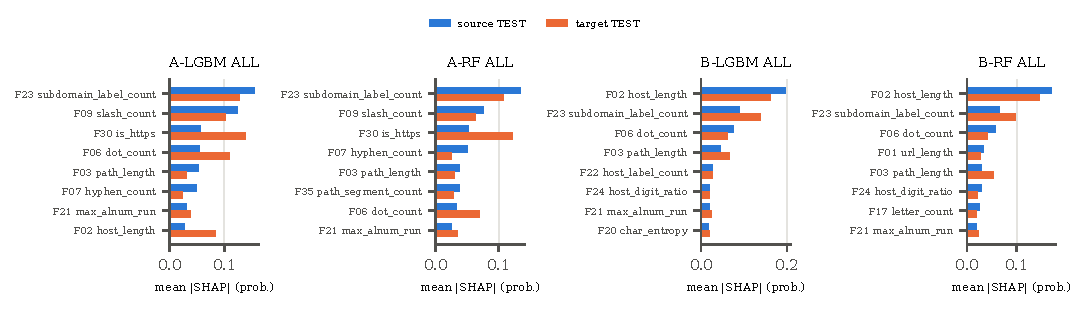
\includegraphics[width=\textwidth]{fig_shap.pdf}
\small Source vs.\ target rank agreement: Spearman $\rho$ \res{rhoMin}--\res{rhoMax}. Descriptive, not causal.
\end{frame}

\end{document}
